\documentclass{article}

\usepackage[super]{nth}
\usepackage{amsmath, amssymb}
\usepackage{hyperref}
\usepackage{graphicx}

\setlength{\textwidth}{6.5in}
\setlength{\textheight}{8.0in}
\setlength{\oddsidemargin}{0in}
\setlength{\evensidemargin}{0in}
\setlength{\parskip}{2ex}
\setlength{\parindent}{0in}

\begin{document}

\section*{Logging Into WebAssign}

\begin{itemize} 

\item Go to \url{www.webassign.net/colorado/login.html} to access the CU WebAssign page.

\begin{center}
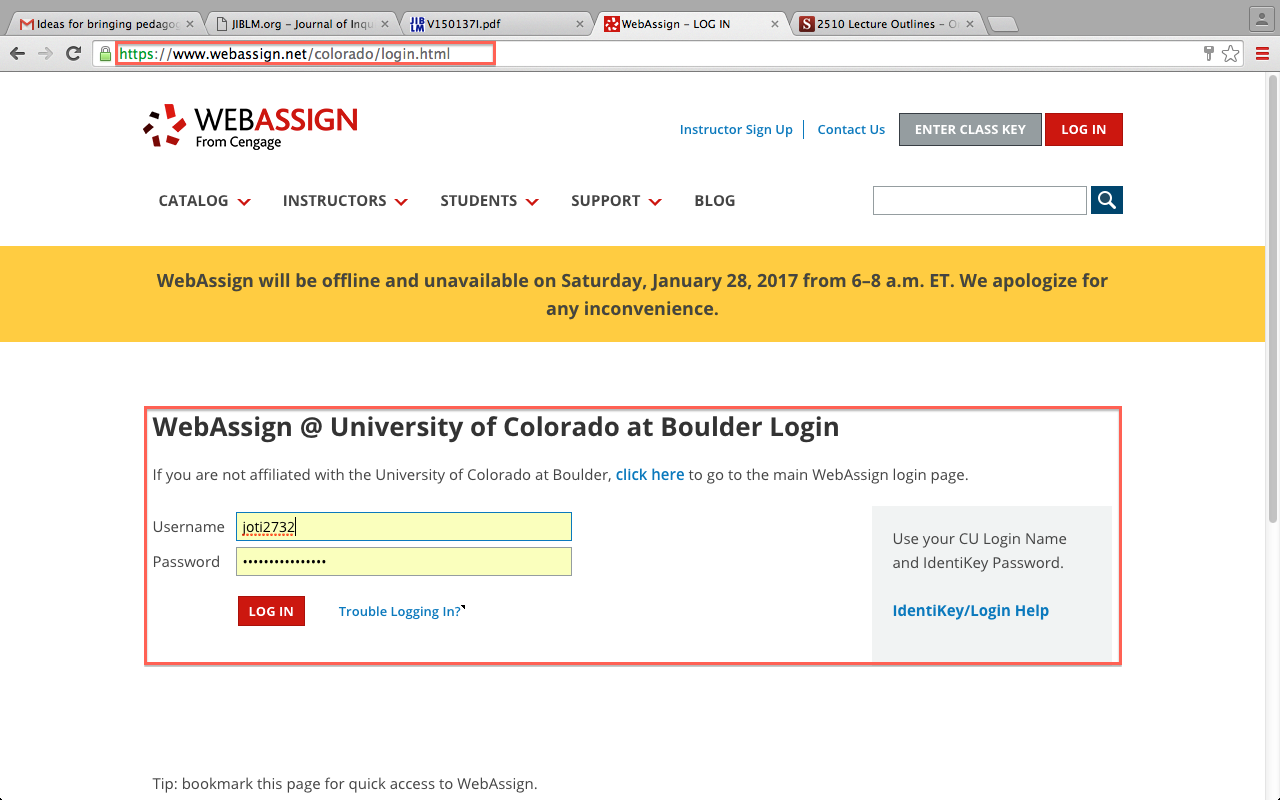
\includegraphics[scale=0.25]{login.png}
\end{center}

\item You should be enrolled in MATH 2510 Section XXX already. If not, you will need to send an email!

\begin{center}
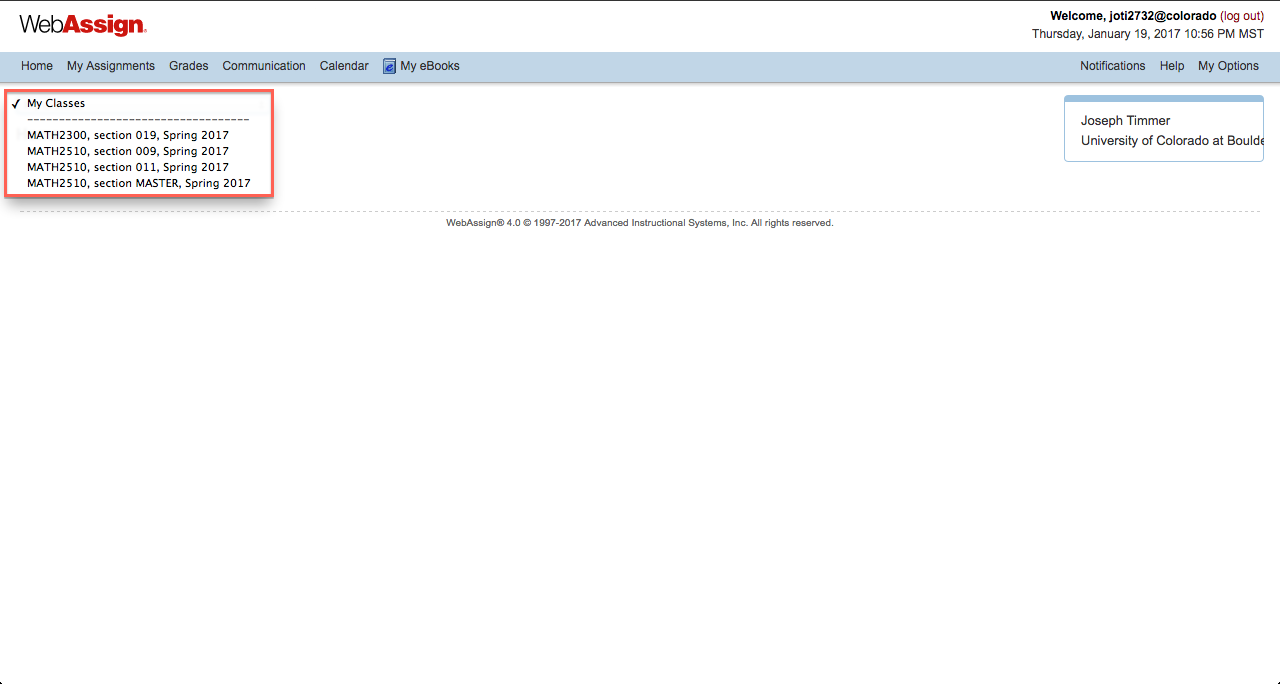
\includegraphics[scale=0.25]{classes.png}
\end{center}

\item If you are not enrolled in a section of MATH 2510, you need to email {\bf math-help@colorado.edu} with your: \begin{enumerate} \item Identikey user name \item CU email address \item The class and section you need to be enrolled in. \end{enumerate}

\item Note when the free trial expires!

\item You will be prompted to either purchase an access code, enter an existing access code or to continue with the free trial. \textbf{You must have a valid access code for this class!}

\begin{center}
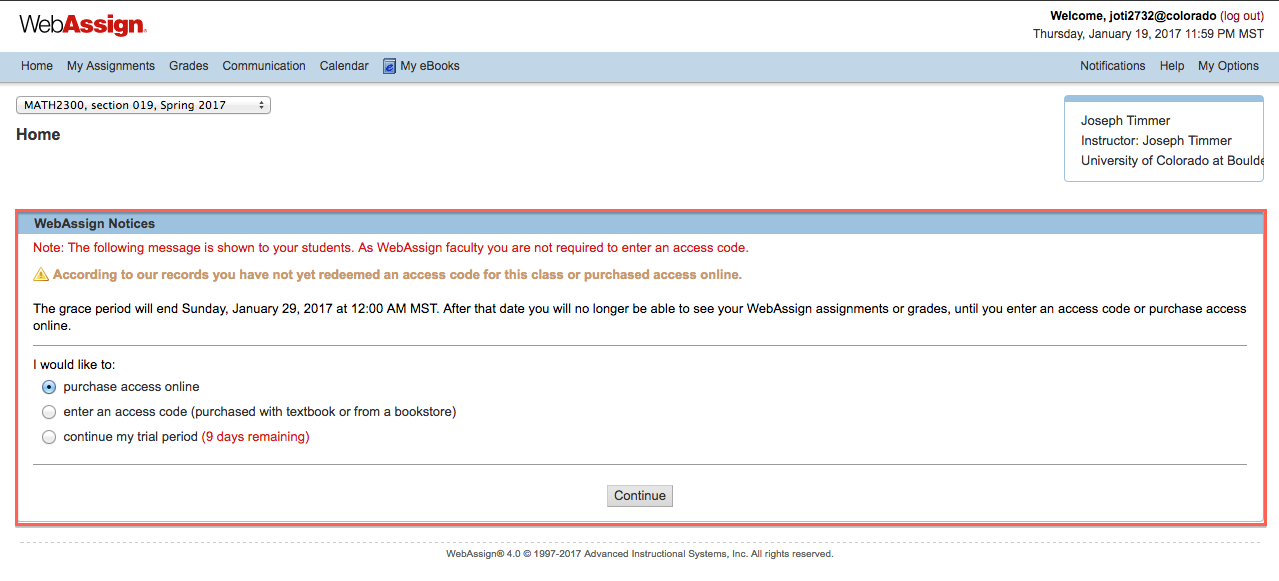
\includegraphics[scale=0.25]{money.png}
\end{center}

\end{itemize}


\section*{Assignments in WebAssign}

\begin{itemize}

\item The Assignments are defaulted to ``Current/Recent" and will display \begin{itemize} \item Assignments that are due in the near future (around 2 weeks) \item Assignments that have recently become past due \end{itemize}

\begin{center}
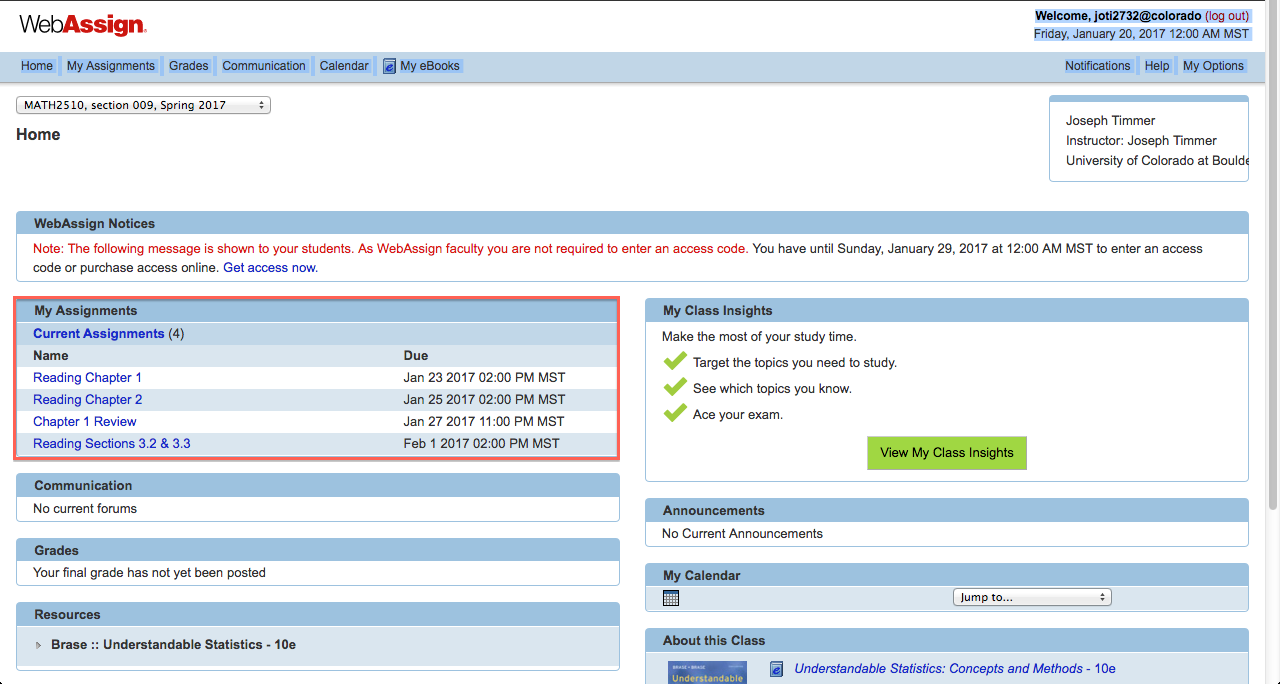
\includegraphics[scale=0.25]{classhome.png}
\end{center}

\item Click on an assignment to view it.

\end{itemize}

\newpage

\section*{Extension Requests}

\begin{itemize}

\item Click on the Assignment you wish to get an extension for. Note it must be past the due date!

\begin{center}
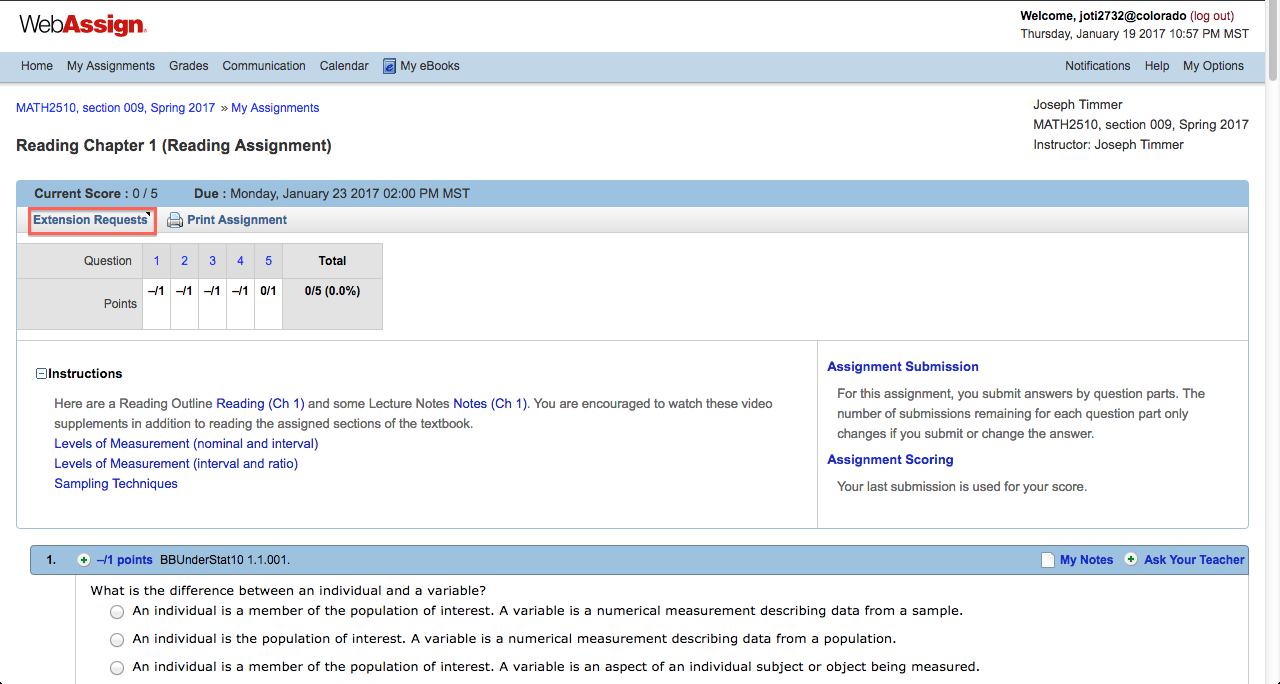
\includegraphics[scale=0.25]{assignment.png}
\end{center}

\item \textbf{For a Reading Assignment, this must be done within 24 hours of the original due date!}

\item \textbf{For a Chapter Review, this must be done within 72 hours of the original due date!}

\end{itemize}

\section*{Problem Interface}

\begin{center}
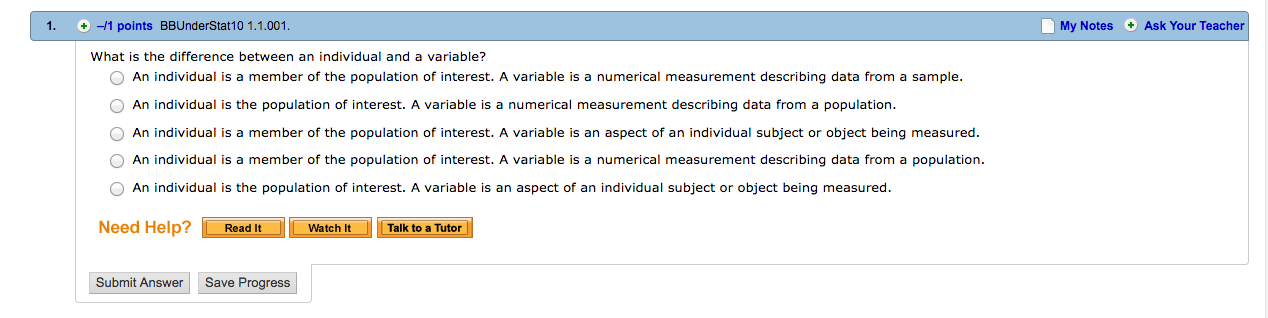
\includegraphics[scale=0.25]{problem.png}
\end{center}

\begin{itemize}

\item Click on the little ``+" to see: \begin{enumerate} \item How many submissions have been used/remain. \item How many points the parts are worth. \end{enumerate}

\begin{center}
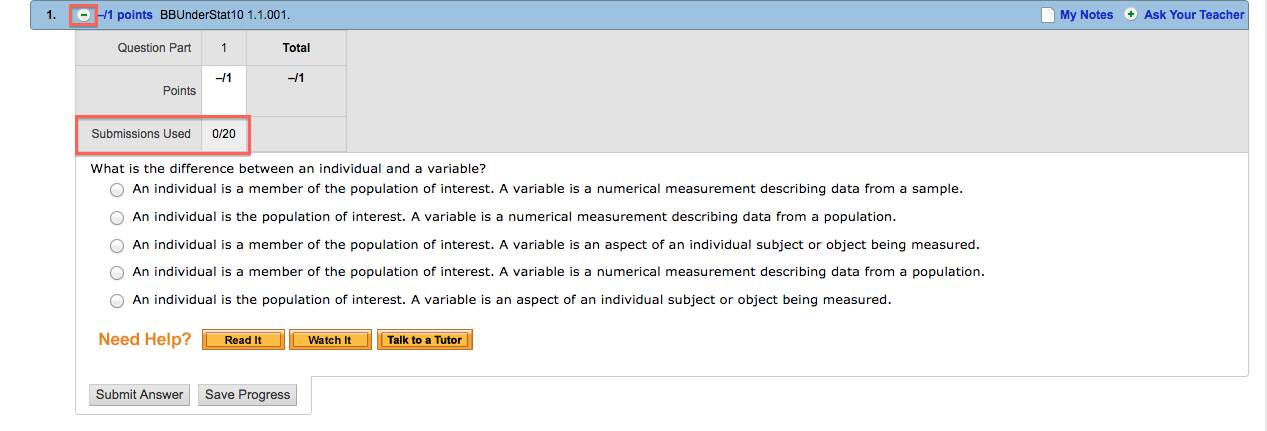
\includegraphics[scale=0.25]{problemplus.png}
\end{center}

\item There are some big yellow buttons to help you when you are stuck!
\begin{enumerate}
\item \textbf{Read It --} Jumps to a relelvant section in the e-book.
\item \textbf{Watch It --} Plays a video about some relevant content.
\item \textbf{Talk to a Tutor} Links to a \nth{3}-Party website that will charge you money!
\end{enumerate}

\begin{center}
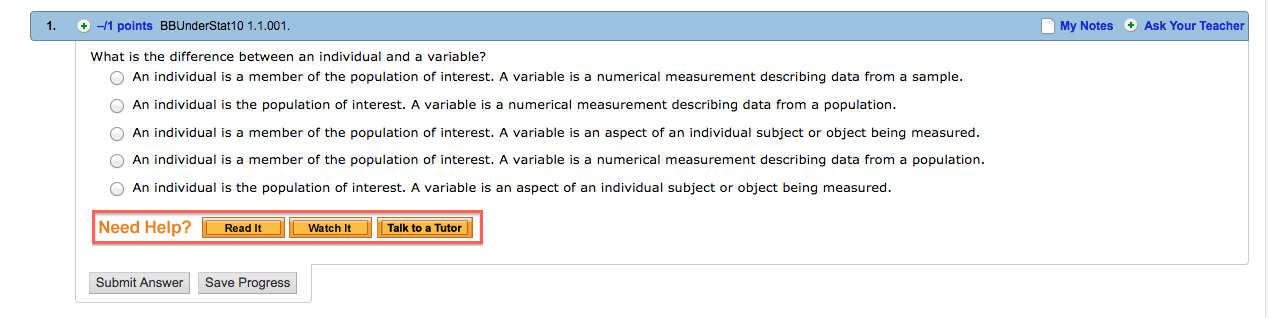
\includegraphics[scale=0.25]{problem-buttons.png}
\end{center}

\item You can also click ``Ask Your Teacher" and send me a question! (response times will vary...)

\begin{center}
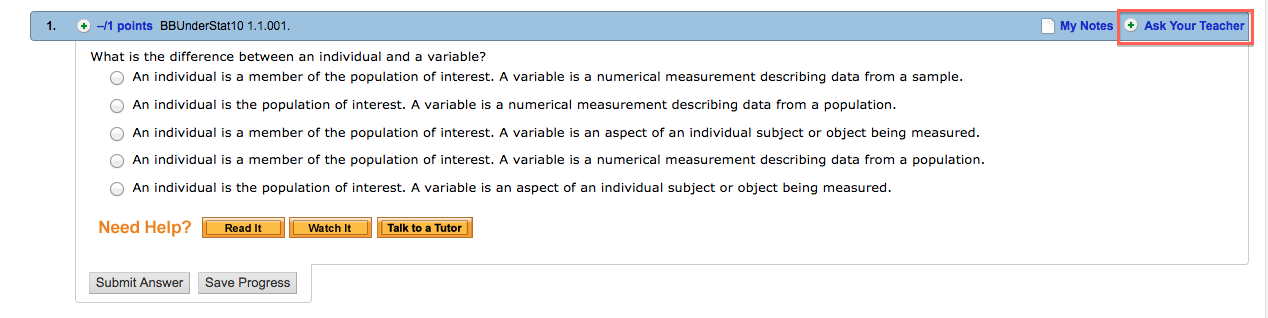
\includegraphics[scale=0.25]{problem-teacher.png}
\end{center}

\item To submit answers, click the submit answer! If you submit an answer and it is wrong, you have used an attempt.

\begin{center}
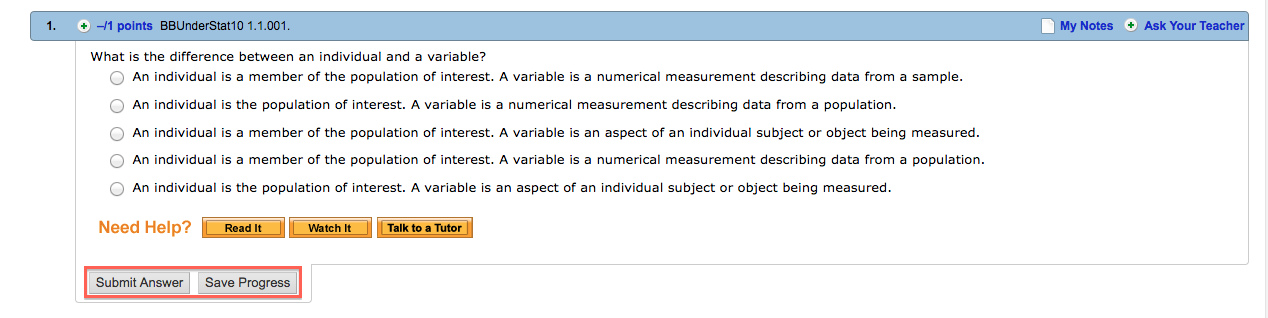
\includegraphics[scale=0.25]{problem-answers.png}
\end{center}

\item Save Progress will merely save the input and not grade the question.
\end{itemize}

\end{document}